\documentclass[tikz,border=10pt]{standalone}
\usepackage{pgfplots}
\pgfplotsset{compat=1.18}

\begin{document}
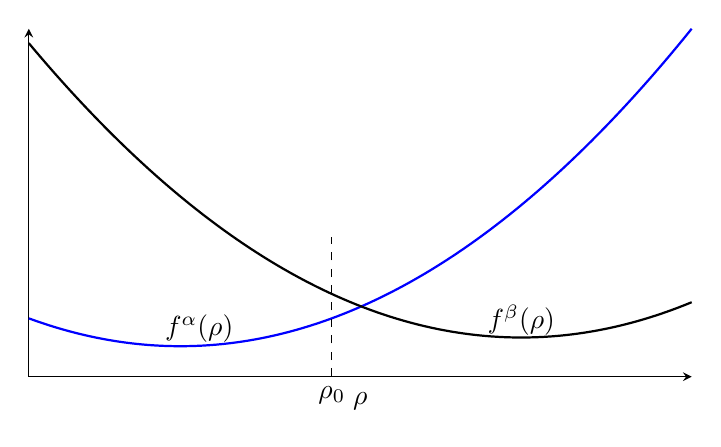
\begin{tikzpicture}
\begin{axis}[
    width=10cm,
    height=6cm,
    axis lines=left,
    xlabel={$\rho$},
    ylabel={},
    xtick=\empty,
    ytick=\empty,
    domain=0:3.5,
    samples=100,
    clip=false
]
\addplot[thick,blue] {(x-0.8)^2+0.7};
\addplot[thick,black] {(x-2.6)^2+0.9};

\node at (axis cs:0.9,1.1) {$f^\alpha(\rho)$};
\node at (axis cs:2.6,1.3) {$f^\beta(\rho)$};

\addplot[dashed] coordinates {(1.6,0) (1.6,3.2)};
\node[below] at (axis cs:1.6,0) {$\rho_0$};
\end{axis}
\end{tikzpicture}
\end{document}
